\section{Chromium}
\label{sec:chromium-chromium}


\subsection{Overview}

% General Information about Chromium
Started in 2008, with more than 2,000 contributors and 25 million lines of code, the Chromium web browser is one of the biggest open-source projects currently existing. Google is one of the main maintainers, but other companies and contributors are also taking part in its development.

% LuCI hierarchy
Chromium relies on \textit{LuCI} as a CI platform~\cite{onlineChromiumGithub}.
It uses more than 900 parallelized builders, each one of them used to build Chromium with different settings (\eg different compilers, instrumented versions for memory error detection, fuzzing, etc) and to target different operating systems (\eg Android, Mac OS, Linux, and Windows). 
% Additionally, some builders are only responsible for running test suites. 
Each builder is responsible for a list of builds triggered by commits made to the project. If a builder is already busy, a scheduler creates a queue of commits waiting to be processed. This means that more than one change can be included in a single build execution if the development pace is faster than what the builders can process. Within a build, we find details about build properties, start and end times, status (\ie pending, success or failure), a listing of the steps and links to the logs. 

% Testing infrastructure
At the beginning of the project, building and testing were sequential. Builders used to compile the project and zip the results to builders responsible for tests. Testing was taking a lot of time, slowing developers' productivity and testing Chromium on several platforms was not conceivable. A swarming infrastructure was then introduced in order to scale according to the Chromium development team's productivity, to keep getting the test results as fast as possible and independently from the number of tests to run or the number of platforms to test. Currently, a fleet of 14,000  build bots runs tasks in parallel. This setup helps to run tests with low latency and handle hundreds of commits per day~\cite{TheChromiumProjects}.

% Figure Decision tree
\begin{figure}[ht]
\centering
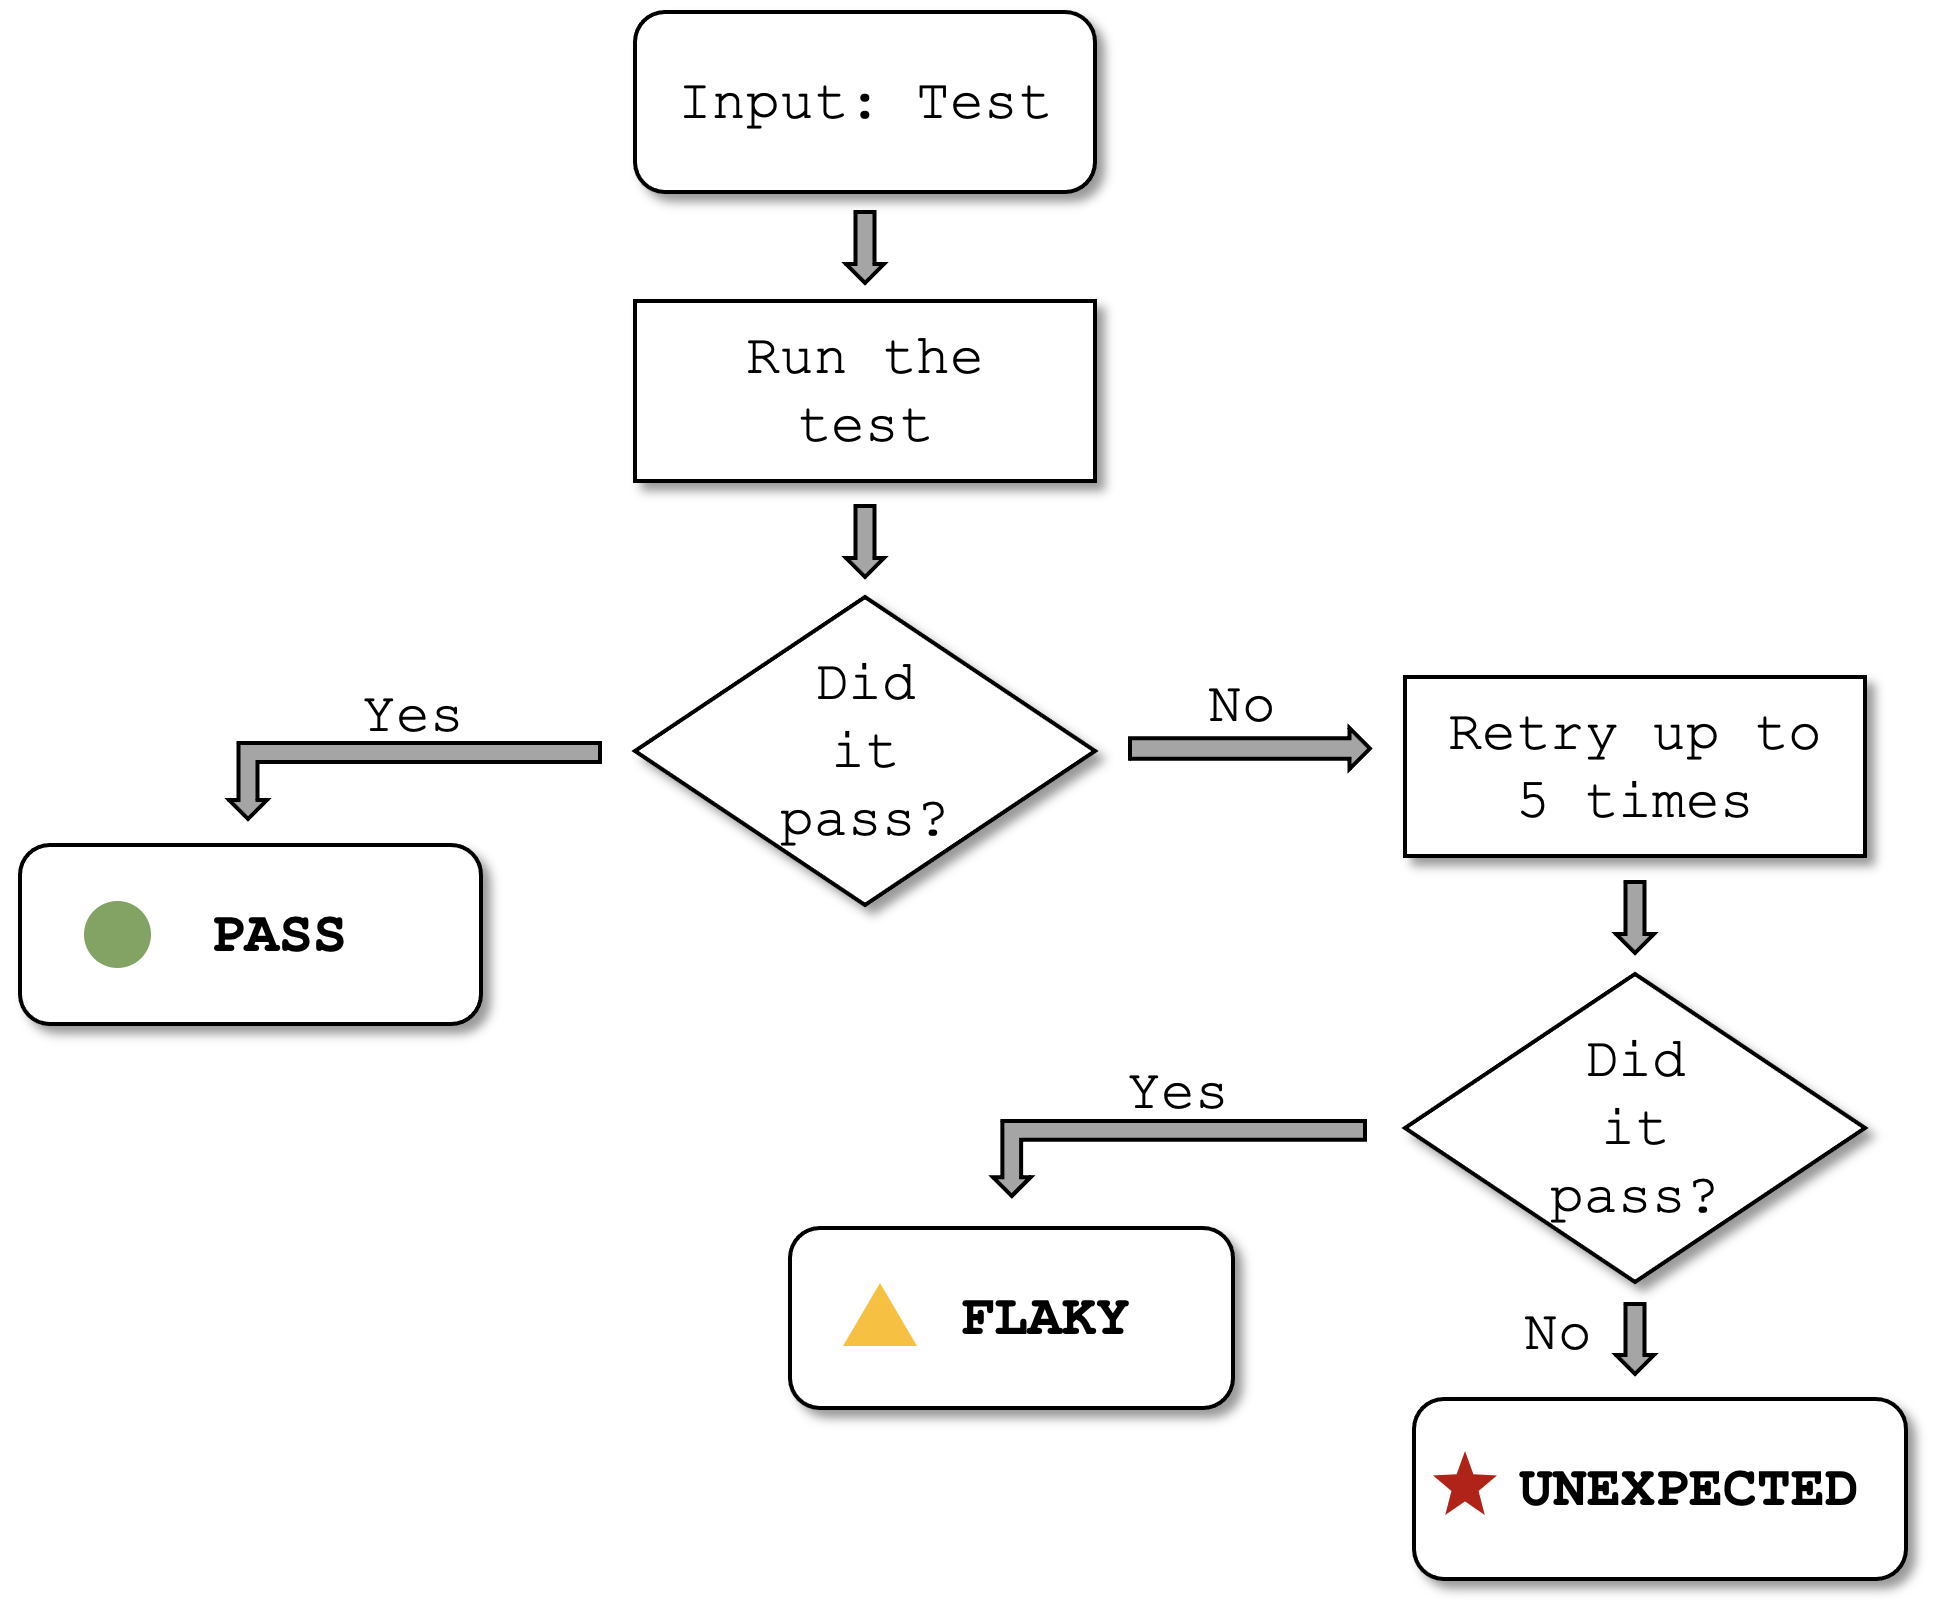
\includegraphics[width=0.8\textwidth]{figures/chromium/gui_process_final.png}
\vspace{-1.0em}
\caption{Decision tree representing how test outcomes are determined in a build by the Chromium CI. 
\includegraphics[scale=0.2]{figures/chromium/pass.png} PASS depicts successful tests, 
\includegraphics[scale=0.2]{figures/chromium/flaky.png} FLAKY depicts tests that passed after failing at least once, while 
\includegraphics[scale=0.2]{figures/chromium/fail.png} UNEXPECTED depicts tests that persistently failed.}
\label{fig:decision-tree}
\end{figure}

% Information about tests
In this study, we focus on testers, \ie builders only responsible for running tests. They do not compile the project: when triggered, they simply extract the build from their corresponding builder and run tests on this version. At the time of writing, we found 47 testers running Chromium test suites on distinct operating systems versions. About 200,000 tests are divided into different test suites, the biggest ones being \textit{blink\_web\_tests} (testing the rendering engine) and \textit{base\_unittests} with more than 60,000 tests each.

% Build results
For each build performed by any tester, we have access to information about test results. Figure~\ref{fig:decision-tree} illustrates the decision process followed by LuCI to determine a test outcome in a specific build. A test is labelled as \textit{pass} when it successfully passed after one execution. In case of a failure, LuCI automatically reruns the test up to 5 times. If all reruns fail, the test is labelled as \textit{unexpected} and will trigger a build failure. In the remaining, we will be referring to \textit{unexpected} tests as \textit{fault-revealing tests}. If a test passes after having one or more failed executions during the same build, it is labelled as \textit{flaky} and will not prevent the build from passing. 


\subsection{Example of a flaky test}

%In this subsection, we discuss an example of a flaky test. By doing so, we seek to give a clearer idea of what Chromium's tests may look like. Furthermore, we show the pieces of information that can be extracted from the tests and used for flakiness detection.

% Figure Decision tree
\begin{figure}[ht]
\centering
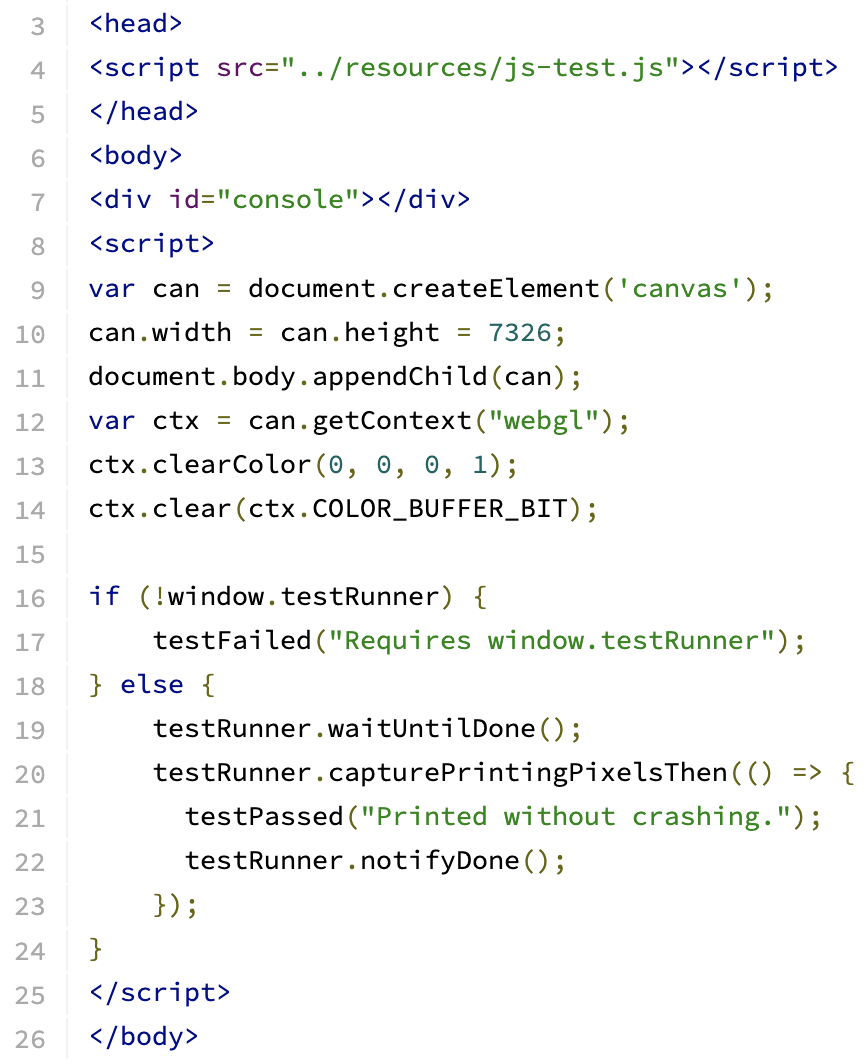
\includegraphics[width=0.8\textwidth]{figures/chromium/flakyTestExample.png}
%\vspace{-1.0em}
\caption{An example of a flaky test caused by a timeout. The test consists of an HTML file \texttt{printing/webgl-oversized-printing.html}, build 119,039 of the Linux Tester. The call to \textsc{waitUntildone()} on line 19 is likely the reason for the failure.}
\label{fig:example}
%\vspace{-0.5em}
\end{figure}

Figure~\ref{fig:example} shows a flaky test found in build 119,039\footnote{https://ci.chromium.org/ui/p/chromium/builders/ci/Linux\%20Tests/119039/} of the Linux Tester. This test, \texttt{printing/webgl-oversized-printing.html}, ensures that no crash happens on the main thread of the rendering process when using the system. Unfortunately, on its first execution, the test failed after 31 seconds. The run status indicates that a \textsc{TIMEOUT} happened. On the second execution, the test passed after 15 seconds and thus was labelled as flaky. In this case, an issue has been opened in Chromium's bug tracking system.\footnote{https://bugs.chromium.org/p/chromium/issues/detail?id=1393294} Developers state that \textit{"this test makes a huge memory allocation in the GPU process which intermittently causes OOM and a GPU process crash"}.

\textsc{Timeout} is a run status that intuitively leads to possible flakiness, as we can easily think of other executions of the same test being completed before reaching the time limit. In addition to this feature, we can also look for hints of flakiness in the source code. As with many UI tests in Chromium, this one is handled by \texttt{testRunner}: a test harness in charge of their automatic executions. We can see the \texttt{testRunner} making a call to \texttt{waitUntilDone()} on line 19. Vocabulary about waits is common in Chromium's web tests. This keyword, for example, could potentially be leveraged by flakiness detectors to classify tests or failures.


% Former place for fig 2: decision tree

